\chapter{Preliminaries}

TODO -- What are the different parts? 

\section{Overview/Preliminaries}
Motion planning is the task of manipulating a robot's configurations so that,
given an initial and goal state or posture, the planner (black box), is able to
create a sequence of actions that gives a feasible or optimal path through the
overarching planning environment, usually referred to as the world space. Thus a
motion planner can be seen as a machine which given an input: a world, and
initial and goal states, produces a sequence of actions to move the robot from
its initial to the desired goal configuration. This plan is then passed on to
the trajectory generator in the system. Generally, planners can be separated
into complete and non-complete planners, meaning that given enough time, all
motion planning problems are solvable, only the solution is NP-Hard. Thus
feasible solutions will have to make a compromise, and a lot of planners in use
today are probabilistically complete, meaning that they converge to a perfect
solution given infinite time. As such time-frames are of no use to us, we
generally have to settle for an approximation bound. There is a difference
between on-line and off-line motion planning, whereas the offline algorithm
plans in a static environment, the online algorithm is run continuously. However
an on-line algorithm can be simulated by running an offline algorithm repeatedly
for short intervals of time. However, this comes with the drawback, that no
guarantee can be made for completing the task at hand \cite{LaValle09}.

\subsection{Building Blocks}

\subsection{The Robot and World Model}

In order to reason about a motion planning problem, a certain reference
framework needs to be built. A mathematical model of the world, and the robot is
necessary for clearly and precisely reasoning about the problem at hand.
Therefore, in this thesis the world space (\modelworld) will be defined as
\[
  \modelworld = \R^2
\]
and obstacles are simply subsets of \modelworld. Likewise, the robot is also a
subset of the world space
\[
  \modelrobot,\, \modelobstacle \subset \modelworld
\]

Next the robot needs to be able to move around in the world space. This is done
through a rigid body transformation on the robot model
\[
  h : \modelrobot\ \rightarrow \modelworld
\]

However, the robot is more than a set of points in the world space. For example
a simple model of a car needs to know its heading as well. This information will
be referred to as the configuration space of the robot
(\modelconfigurationspace). For a simple car model this can be encoded in a
simple three dimensional vector holding the \(x\), \(y\), and \(\theta\)
parameters, like so
\[
  \modelconfigurationspace \subset SO(2),
\]
which encompass all the states the robot can be in during, and \(SE(2)\) stands
for \textit{Special Euclidean two}, and is defined as \(SE(2) = \R^2 \times
\mathsf{S}\).

\subsubsection{Configuration Space}

TODO -- fix shite!

The configuration space is a general abstraction used as a model for a wide
variety of motion planning problems. It is a manifold that arise from the
transformations applied to the robot. If the robot has n-degrees of freedom, the
set of transformations is usually a manifold of dimension n. This manifold is
called the configuration space of the robot, and is shortened
\modelconfigurationspace{}. Thus in order to solve a motion planning problem, a
search must be performed in the configuration space. Thus the motion planning
problem is now made into a question of finding the best path to traverse the
given manifold\cite{Lav06}.

Using generalized coordinates, the configuration of a robot can be modeled as a
vector with n variables for the position in the configuration space, in
literature this space is usually denoted by \modelconfigurationspace{}. As is
most common, the robot is modeled as a rigid body, in which two bodies cannot
overlap, thus points in the configuration space is separated into two sets. One
set for which the robot configuration overlaps with another object in the
configuration space, and is called \modelconfigurationspaceobst{}, and given
that the world space is represented as \modelconfigurationspace{}, the collision
free space is the given as, \(\modelconfigurationspacefree =
\modelconfigurationspace \setminus \modelconfigurationspaceobst\). The obstacle
region of the world space can be represented in a number of ways, but we will
stick to polygonal models of the obstacle space.

\subsection{Action Space}

Now that the configuration space, and how the robot model can move in the world
space is defined, the next concern is to control the movement of the robot
model, and this is where the \textit{action space} comes in. The action space is
the set of actions that can be applied at any given state the robot is in. Thus
one can model the action space as a function of the robot's state.\ e.g.
\[
  \modelactionspace(x) = \set{u \in \modelactionspace \mid \modelactionspace(x)
    \neq \emptyset }
\]

\subsection{Initial and Goal States}

A planning problem needs to have an initial condition, and a goal. It is normal
to define an initial state and a goal state as a starting and an ending point of
a planning problem. Where both the initial, and goal states can be sets of
states, meaning that it is not necessary to arrive specifically at the target
point.

\subsection{Model}

A mathematical model of the planning problem.

The \rrtfunnel\ motion planning algorithm is discrete, therefore only the
discrete motion planning formulation will be defined. Note however that there is
a rich literature surrounding the continuous case also. In fact a lot of
discrete motion planners have simply been adapted from a continous analog. Also
even though the planner itself is discrete, the configuration space can be -- and
is in this thesis -- continuous.

\subsubsection{Discrete}

Let \(\mathcal{X}\) be the discrete state space, and \(\mathcal{U}(x)\) be the
set of actions available at each point \(x \in \mathcal{X}\). State transition:\
\[
  x_{k+1} = f(x_k, u_k)
\]

\subsubsection{Path and Trajectory}

A motion plan takes the form of a path, or a trajectory. This is represented as
a function \(\phi(\alpha) \colon [0,1] \rightarrow \mathcal{X}\), where
\(\mathcal{X}\) is the configuration space of the vehicle. If the
control-execution time is considered, then the explicit model of vehicle
kinematics and/or dynamics, as well as the dynamics of the possible obstacles.
Then the trajectory is represented as a time-parameterized function of the kind
\(\pi(t) \colon [0,T] \rightarrow \mathcal{X}\), where \(T\) is the planning
horizon. Unlike the path, the trajectory describes how the configuration of the
vehicle evolves over time.

Initial and Goal States. A path is a function f \ldots

\section{Planning Under Uncertainty (Decision Theoretic Planning)}

All real life motion planning problems are faced with some level of uncertainty,
as errors can arise from a multiple of sources, whereas the most prevalent ones
are uncertainty in:
\begin{enumerate}
\item motion
\item sensing
\item the environment
\end{enumerate}
Thus the exact system state is never exactly known. Therefore planning under
uncertainty is done in a belief space, which is a description of the state space
using probability distributions. Planning is done in the information space, as
opposed to the state-space. Uncertainties in prediction and the current state
exist. The information space is a general structure for working with plans under
conditions of uncertainty. Thus planning can be done mostly as it is done in a
state space, albeit in a higher dimension. Thus the state transition function
can be written as
\[
  \phi_{k+1} = f_{\mathcal{I}}\left( \phi_k, \mu_k, y_{k+1} \right)
\]

\subsection{A Model of Uncertainty}

If the discrete state space model is expanded to include \(\theta\) as the
space of nature actions, and \(\ theta_k\) is the action selected by nature at
step k, then a transition is modeled as
\[
  x_{k+1} = f(x_k,u_k,\theta_k)
\]
As the actions of nature are not available beforehand, that is -- \(\theta_ k\)
is not given, thus we have
\[
  X_{k+1} = \set{ x_{k+1} \ in X \mid \exists\theta_k \in \Theta(x_k,u_k)
    \text{such that } x_{k+1} = f(x_k,u_k,\theta_k)}
\]\cite{Lav06}.

\subsection{A Plan under Uncertainty}
Since it Expected-case analysis. Worst-case analysis.

\subsection{Trajectory planning}

The \rrtfunnel\ algorithm relies on validating robust trajectories as motion
primitives for the planner. However, solving for a valid initial trajectory is a
hard control problem in itself. Thus in order to surmount this obstacle

\subsection{Reachable sets}

Of particular interest to the \rrtfunnel\ algorithm is the reachable set. A
reachable set is all the configurations that the robot can be in if started from
a particular point in the world space. Had there been no constraints on the
movement of the robot the reachable set would simply be the entire configuration
space. However, the simple car model has both \textit{kinodynamic} and
\textit{non-holonomic} constraints. This leads to the car not necessarily being
able to reach all the states in the state-space from a given starting position.
At least not given a time frame. This idea is important as it leads to the
funnel definitions that makes up the backbone of this thesis. As an example, the
reachable set for the \textit{Dubins car} will look like this

\begin{figure}
  \centering
  \documentclass[border=3mm,tikz]{standalone}
\begin{document}
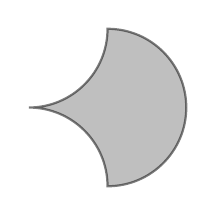
\begin{tikzpicture}
  \draw [black, fill=gray, opacity=.5, thick] (0,0) arc (270:360:1cm) -- (1,1) arc (90:-90:1cm)  -- (1,-1) arc (0:90:1cm);
\end{tikzpicture}
\end{document}
\end{figure}

\subsection{Motion primitives}

A motion primitive is a constant action applied over fixed time intervals. It is
one or more actions collected into one distinct action, usually with a goal. As
an example, the action the \textit{Dubin's car} employs is steering the angle of
the wheels. Setting the angle to a constant over a time interval can be a motion
primitive, however, it is more easily thought of as a collection of actions over
time, which embodies one bigger, more abstract action. For the car this could be
\textit{go straight}, \textit{turn left}, etc. In this way, a collection of
actions can be thought of as one simple action.

\section{Misc}

\begin{table}
  \begin{tabular}{c c c p{4cm}}
    \hline
    \hline
    Algorithm Group & Technique & Variations & Description \\
    \hline
                    &  Dijkstra's Algorithm & &Algorithm for finding the shortest weighted path in a graph.\\
                    &  \\
    Graph Search               & & D* & Capable of planning paths in unknown, partially known, and changing environments in an efficient, optimal, and complete manner..\\
                    & A* Family & Focused-D* & Informed-incremental heuristic search.\\
                    & & D*-Lite & Simpler to implement that Focused D*, slightly slower performance.\\
    \hline
                    & RRT-implementations \\
                    & & RRT\\
                    & & RRT*\\
    Sampling based Planners& & RRT*-Smart\\
                    & & RRT-SLAM\\
                    & & CC-RRT\\
                    & PRM \\
                    & & BRM & A road-map implementation that plans in belief space in order to handle uncertainties in the planning model.\\
    \hline
    Numerical Optimization &  Function Optimization \\
    \hline
  \end{tabular} 
\end{table}

\section{Planning with Funnels}

A \textit{Funnel} is a parametrization of the reachable set of a dynamical
system. This means that a \textit{Funnel} holds all the states the dynamical
system can be in during a planning task. Mathematically we can define the
reachable set of the system as
\[
  \bar{x}(0) \in \mathcal{X}_0 \Rightarrow \bar{x}(t) \in F(t), \forall t \in
  \sqb{0,T}
\]
where \(\mathcal{X}_0\) is the set of initial conditions, \(\sqb{0,T}\) the time
interval, and \(F(t)\) is the set of states that the system can be in at time
\(t\). Although this thesis concerns itself with approximating the reachable set
through \textit{Lyapunov} functions, a useful analogy is imagining the funnel
created through \textit{Monte-Carlo} simulation, where the \textit{Funnel} would
be the set of all the paths traversed by the dynamical system at hand. For a
simple car model, this could look similar to:

\begin{figure}
  \centering
  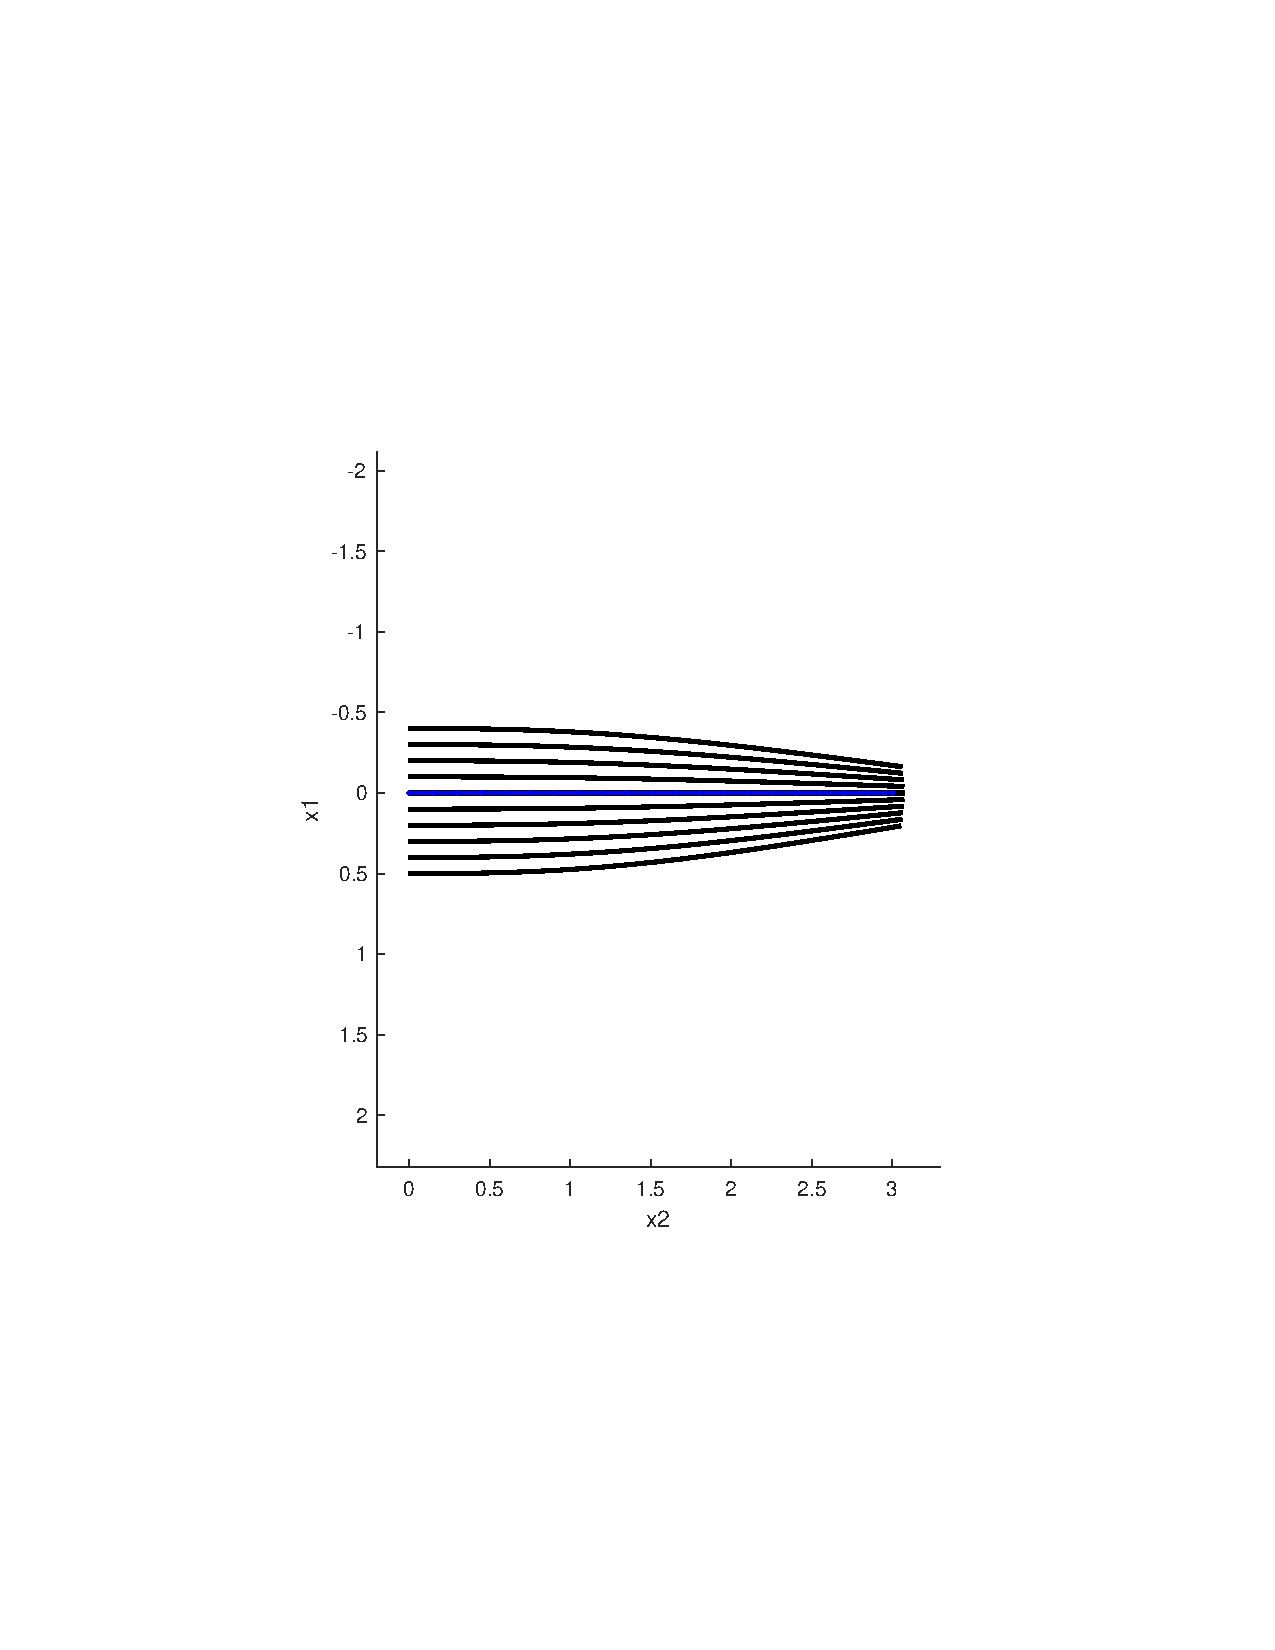
\includegraphics[scale=.5]{figures/preliminaries/montecarlofunnel}
  \caption{The simulation of N paths starting from a random point in the
    interval \(\sqb{-1,1}\), and controlled with a LQR controller.}
\end{figure}

In this thesis a \textit{Funnel} will refer to the \textit{outer approximation
  of forwards reachable sets} parameterized by a \textit{Lyapunov function}.


\section{Funnels}
\label{sec:Funnels}

TODO -- Create a timeline of these papers.

The term \funnel\ first appears in \cite{masonMechanicsManipulation1985}. The
\funnel{} definitions in this thesis is taken from a series of articles on
\funnel{}'s \cite{tobenkinInvariantFunnelsTrajectories2010}
\cite{tedrakeLQRtreesFeedbackMotion2009} \cite{majumdarRobustOnlineMotion2013}
\cite{majumdarFunnelLibrariesRealtime2017}
\cite{ahmadiDSOSSDSOSOptimization2017}, with the main focus being on
\cite{majumdarFunnelLibrariesRealtime2017}. Here a \funnel\ is mathematically
defined as
\[
  \bar{x}(0) \in \mathcal{X}_0 \implies \bar{x}(t) \in F(t), \forall t \in
  \sqb{0,T}
\]
where \(\mathcal{X}_0\) is the set of initial conditions, \(\sqb{0,T}\) the time
interval, and \(F(t)\) is the set of states that the system can be in at time
\(t\). Although this thesis concerns itself with approximating the reachable set
through \textit{Lyapunov} functions. A useful analogy is imagining the funnel
created through a \textit{Monte-Carlo} simulation, where the \funnel{} would be
the set of all the paths traversed by the dynamical system at hand. For a simple
car model, this could look similar to:

\begin{figure}
  \centering
  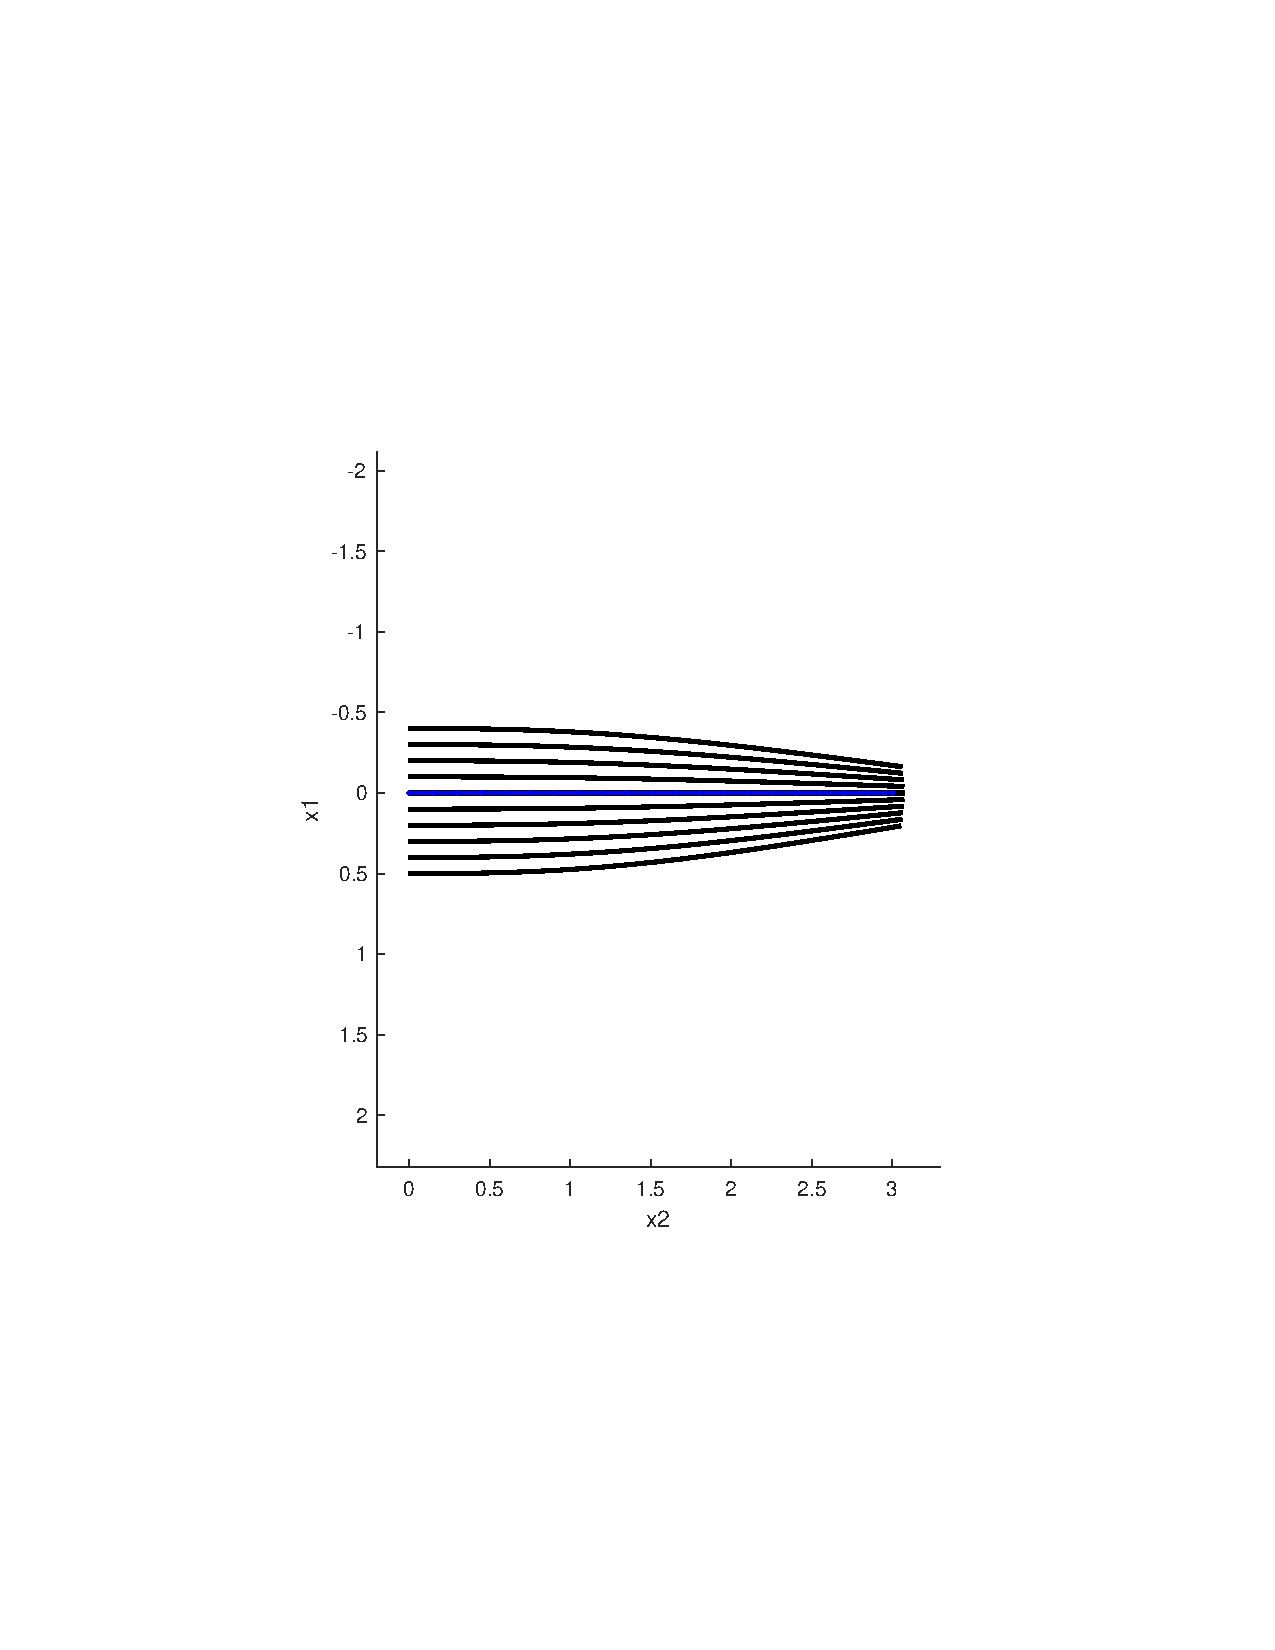
\includegraphics[scale=.5]{figures/preliminaries/montecarlofunnel}
  \caption{The simulation of N paths starting from a random point in the
    interval \(\sqb{-1,1}\), and controlled with a LQR controller.}
\end{figure}

\subsection{Lyapunov Functions}

A \textit{Lyapunov function} for an autonomous dynamical system is defined as a
scalar function \(V: \R^n \rightarrow \R\), with continuous first derivatives,
is locally positive definite, and \(\Delta V \dot g\) is also locally negative
definite. The \textit{Lyapunov functions} can then be used to prove the
\textit{Lyapunov stability} of the dynamical system. If \(\dot{x} = f(x)\) is a
dynamical system, and \(\dot{V}\) is the time derivate of the
\textit{Lyapunov-candidate function} \(V\), then:
\[
  \dot{V}(x) = \frac{d}{dt}V(x(t)) = \frac{\partial V}{\partial x} \cdot
  \frac{dx}{dt} = \Delta V \cdot \dot{x} = \Delta \cdot f(x)
\]

\subsection{Lyapunov Stability}

A function being stable in the sense of \textit{Lyapunov}, is defined as: Given
the autonomous nonlinear dynamical system
\[
  \dot{x} = f(x(t)), \, x(0) = x_0
\]
with \(\x(t)\) denotes the state vector of the system, with \(x(t) \in
\mathcal{D} \subseteq \R^n\). \(\mathcal{D}\) is an open set containing the
origin, and \(f \colon \mathcal{D} \rightarrow \R^n\) continous on
\(\mathcal{D}\). Suppose that \(f\) has an equilibrium at \(x_e\) so that
\(f(x_e) = 0\), then this equilibrium is \textit{Lyapunov stable} if for every
\(\epsilon > 0\) there exists a \(\delta > 0\) such that if \(\left \lVert x(0)
  - x_e \right \rVert < \delta\) then for every \(t \geq 0\) we have \( \lVert
x(t) - x_e \rVert \leq \epsilon\).

Conceptually this means that a solution starting out in the vincinity of the
equilibrium (\(\delta\)), will remain close (\(\epsilon\)) to it. Also note that
this must be true for any \(\epsilon\) one may choose. (semicite wikipedia?).

\subsection{Lyapunov's second method for stability}

\textit{Lyapunov's} second method (also referred to as \textit{Lyapunov's}
direct method) for stability makes use of the \textit{Lyapunov} function \(V\).
If given a dynamical system of the form \(\dot{x} = f(x)\) having a point of
equilibrium at \(x = 0\). Consider a function \(V(x) \colon \R^n \rightarrow
\R\), such that
\begin{align*}
  V(x) &= 0 \text{ if and only if } x = 0 \\
  V(x) &> 0 \text{if and only if} x \neq 0 \\
  \dot{V}(x) &= \frac{d}{dt}V(x) = \sum_{i=0}^{n} \frac{\partial V}{\partial x_i} f_i(x) \leq 0 \text{ for all values of } x \neq 0. \\
\end{align*}
Then \(V(x)\) is called a \textit{Lyapunov function} candidate and the system is
stable in the sense of Lyapunov. (semicite wikipedia).

The following sections \ref{subsec:LaSalle's invariance principle},
\ref{subsec:LaSalle's invariance principle}, \ref{subsec:Lyapunov analysis for
  linear systems}, are based on the lecture notes from
\cite{tedrakeUnderactuatedRoboticsAlgorithms2019}, and are adapted slightly for
presentation in this thesis.

\subsection{LaSalle's invariance principle}
\label{subsec:LaSalle's invariance principle}

\textit{LaSalle}'s invariance principle formalizes the convergence of a
dynamical system to an invariant set, rather than to a fixed point. Defined as:
Given a system \(\dot{x} = f(x)\) with \(f\) continuous. If we produce a scalar
function \(V(x)\) with continous derivatives for which over an open subset
\(\mathcal{B} \in \R^n\) we have
\begin{align*}
  V(x) \geq 0, \; \dot{V}(x) \leq 0,
\end{align*}
and \(V(x) \rightarrow \infty\) as \(\norm{x} \rightarrow \infty\), then \(x\)
will converge to the largest \textit{invariant set} where \(\dot{V}(x) = 0\).
Where an \textit{invariant set}, \(\mathcal{G}\), of the dynamical system is a
set for which \(x(0) \in \mathcal{G} \implies \forall t > 0,\, x(t) \in
\mathcal{G}\). Meaning that once you enter the region of invariance, you never
leave; which will be important for our funnel calculations later on.

\subsection{Lyapunov analysis with convex optimization}
\label{subsec:Lyapunov analysis with convex optimization}

One of the primary limitations in Lyapunov analysis is that it is potentially
very difficult to come up with suitable \textit{Lyapunov} function candidates
for underactuated systems. Even if given a \textit{Lyapunov} function, simply
checking that the \textit{Lyapunov} conditions hold for all \(x\) can be
difficult. Imagine checking that \(\dot{V}\) is strictly negative for all \(x\),
except at the origin, if \(\dot{V}\) is some complicated nonlinear function over
a vector \(x\). However with recent advances in convex optimization
\cite{parilloStructuredSemidefinitePrograms}, there now exists the opportunity
to numerically search for these functions.

A natural approach to a numerical algorithm for verifying \textit{Lyapunov}
stability could be to evaluate \(V\) and \(\dot{V}\) at a large number of points
and check that \(V\) is positive, and that \(\dot{V}\) is negative. Which
\href{https://github.com/RobotLocomotion/drake/blob/master/systems/analysis/test/lyapunov_test.cc}{does
  in fact work}. But in reality we can do better, using optimization algorithms
which rigourously checks these conditions \textit{for all \(x\)}, without the
need for dense sampling. Which in actuality enables us to search for
\textit{Lyapunov functions} in an infinite function space (which is what makes
up the space of all \textit{Lyapunov} functions).

\subsection{Lyapunov analysis for linear systems}
\label{subsec:Lyapunov analysis for linear systems}

\begin{theorem}
  Given a linear system of the form \(\dot{x} = Ax\) if one can find a
  \textit{Lyapunov function}
  \[
    V(x) = x^{T}Px, \; P = P^{T} \succeq 0
  \]
  where \(\succeq\) means that the matrix is \ac{PSD}.
  This also satisfies
  \[
    \dot{V} = x^{T}PAx + x^{T}A^{T}Px \succeq 0.
  \]
  Then the origin is globally asymptotically stable.
\end{theorem} \cite{tedrakeUnderactuatedRoboticsAlgorithms2019}

For the linear case the existence of a quadratic \textit{Lyapunov} function is a
necesary and sufficient condition. Furthermore, a \textit{Lyapunov} function can
always be found by finding the positive definite solution to the matrix Lyapunov
equation
\begin{equation}
  \label{eqn:linearlyapunov}
  PA + A^{T}P = -Q
\end{equation}
for any \(Q = Q^{T} \geqslant 0\).

\subsection{The connection between Lyapunov analysis and convex optimization}

The first connection between Lyapunov analysis and convex optimization will be a
\ac{SDP}-program. In fact the Lyapunov conditions for a linear system can be
formulated in the form of an \ac{SDP} - which is a form of convex optimization.
For any problem formulated as an \ac{SDP} there exists an efficient -- and
optimal -- solution, barring numerical difficulties.

\subsection{Numerical convex optimization}

\subsubsection{Linear programming}

\subsubsection{Semidefinite programming}

A wide variety of nonlinear convex optimization problems can be formulated and
efficiently solved as \ac{SDP}s. In control theory, semidefinite programming is
a method for numerically finding the optimal solution of a linear matrix
inequality. It is concerned with the optimization of a linear objective function
over the intersection of the \textit{cone} of positive semidefinite matrices
with an affine space.

A convex cone is a subset of a vector space over an ordered field that is closed
under linear combinations with positive coefficients.

\begin{figure}
  \centering
  \includegraphics[scale=.5]{figures/preliminaries/Convex_cone_illust}
  \caption{A convex cone (light blue). Inside of it, the light red convex cone
    consists of all points \(\alpha x + \beta y \) with \(\alpha,\, \beta > 0\),
    for the depicted \(x\) and \(y\). The curves on the upper right symbolize
    that the regions are infinite in extent.
    \cite{alexandrovConvexConeIllust2019}}
\end{figure}

A semidefinite program can solve all problems of the form:
\begin{align*}
  \text{minimize } &TrCX \\
  \text{subject to } &TrA_{i}X = b_{i} \text{for all i } = 1,\ldots,m\\
                   &X \succeq 0
\end{align*} 
where \(X \in S^n\), with \(S^n\) being the space of real symmetric \(nxn\)
matrices. The vector \(b \in \R^m\), and the matrices \(A_i \in S^n\), and \(C
\in S^n\) are given problem
parameters\cite{wolkowiczHandbookSemidefiniteProgramming2000}.

\subsection{A simple example}
\label{subsec:A simple example}

\begin{align*}
  \min{a} \text{subject to}
  \begin{bmatrix}
    a & 0 \\
    0 & 1 \\
  \end{bmatrix}
  \succeq 0
\end{align*}\cite{tedrakeUnderactuatedRoboticsAlgorithms2019}

The linear Lyapunov example from above \ref{subsec:Lyapunov analysis for linear
  systems}, can also be formulated as an \ac{SDP} like so:
\begin{align*}
  \text{find p, subject to } P \succeq 0, \; PA + A^{T}P \preceq 0.
\end{align*}\cite{tedrakeUnderactuatedRoboticsAlgorithms2019}

This formulation then provides the ground for an automatic search for a
\ac{LQR}-controller. Shown below, is also how one can make it robust to bounded
uncertainties.

Given the system \(\dot{x} = Ax\), where \(A\) is unknown, with bounded
uncertain parameters. This set can be described by writing \(A\) as an uncertain
linear combination of known matrices, e.g:
\[
  A = \sum_{i} \beta_{i}A_{i}, \; \sum_{i}\beta_{i} = 1, \; \forall i,\beta_{i}
  > 0
\]
Geometricall the formulation descibes a polygon in the \(A\) space, with each
vertice being one of the \(A_{i}\) which is used to describe a as a linear
combination.

\begin{figure}
  \centering
  % 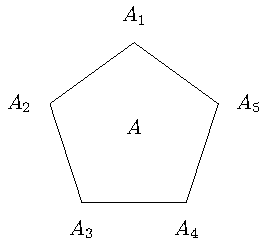
\includegraphics{figures/funnel/linearuncertainlyapunov}
  \documentclass[tikz]{standalone}
\usetikzlibrary{shapes.geometric}

\begin{document}
    \begin{tikzpicture}
      \foreach \a in {5}{
        \node[regular polygon, regular polygon sides=\a, minimum size=3cm, draw] at (\a*4,0) (A) {};
        \node[circle, label=above:\(A_1\)] at (A.corner 1) {};
        \node[circle, label=left:\(A_2\)] at (A.corner 2) {};
        \node[circle, label=below:\(A_3\)] at (A.corner 3) {};
        \node[circle, label=below:\(A_4\)] at (A.corner 4) {};
        \node[circle, label=right:\(A_5\)] at (A.corner 5) {};
        \node[circle, label=\(A\)] at (20,-.35) {};
      }
    \end{tikzpicture}
\end{document}
  \caption{Illustration of the search space. Adapted from~\cite{tedrakeUnderactuatedRoboticsAlgorithms2019}}
\end{figure}


This problem, once formulated can the be sent to an automatic \ac{SDP}-solver,
such as \textit{MOSEK}\cite{mosek}, which is used in this thesis.

This example is important as it provides a way in which to search an infinite
function space (The Lyapunov functions) -- numerically -- for a function which
fullfills our constraints, and solves the problem. Furthermore, the solution is
optimal as long as the problem is convex. Downside, however, is that this method
only works on linear systems, and the problem at hand in this thesis is
nonlinear.

Fortunately, with the advent of \ac{SOS} programming, it is now possible to
formulate the search for Lyapunov functions as a convex optimization problem.

\section{SOS}

The tools to search for a Lyapunov function for a nonlinear system relies on the
algebraic geometry theory of \ac{SOS}, which is about representing
\textit{non-negative polynomials} as a sum of squares of polynomials. In short,
if one can write a polynomial \(p\) with indeterminates \(x_1,x_2,\ldots,x_n\)
is \ac{SOS} if
\[
  p(x) = \sum_{i=1}^{m}g_i^2(x)
\]
for \(g_i \in \P\), where \(\P\) is the space of polynomials. The clue here is
that every form that is \ac{SOS} is also a positive polynomial, although the
converse is not necessarily true\cite{majumdarFunnelLibrariesRealTime2016}.

This is an important detail, as the numerical search for Lyapunov functions can
only verify \ac{SOS}-polynomials, and as such there will be a \textit{gap} in
the Lyapunov functions we can find and verify, and the best Lyapunov functions
for the task, as it is no guarantees that a \ac{SOS}-Lyapunov function will be
the optimal function for the task.

\ac{SOS} is the theory of

As seen in section~\ref{subsec:A simple example}, if one is able to

\acl{SOS} polynomials are

\acl{SOS} programming is

\cite{parilloStructuredSemidefinitePrograms},

\subsection{SOS programming}

The procedure used for searching the space of all positive Lyapunov functions
which can be written as a sum of squares is \ac{SOS} programming.
With~\cite[Parillo's]{parilloStructuredSemidefinitePrograms}, work, there now
exists an efficient way of restructuring a \ac{SOS} program into an \ac{SDP}
program, solve it, then convert it back, and get the sought solution polynomial.

\ac{SOS} programming relies on the ability to write a SOS polynomial in the form
\begin{align*}
  p(x) &= s{(x)}^{T}Qs(x)\\
\end{align*}
where \(p(x)\) is a \ac{SOS} polynomial, and \(Q\) is \ac{PSD}, and \(s(x)\) is
a vector of \textit{monomials} -- meaning that its elements are the terms in a
polynomial, like so
\[
  s(x) = \begin{bmatrix} 1 \\ x \\ y \\ x^2 \\ xy \\ y^2 \end{bmatrix}
\]
where \(s(x)\) is a monomial in \(x\) and \(y\) of order two.In general \(s(x)\)
is a monomial with degree less than or equal to half that of
\(p(x)\)\cite{parilloStructuredSemidefinitePrograms}\label{monomialdegree}. The
condition that \(s(x)\) is \ac{SOS} is much more \textit{computationally
  tractable} than a nonnegativity
constraint~\cite{parilloStructuredSemidefinitePrograms}. The methodology used in
the \ac{SOS} program in this thesis is based on the relaxation
from~\cite{parilloStructuredSemidefinitePrograms}, which in turn is based on the
\textit{Positivstellensatz} from algebraic geometry. In this type of problem the
interest is in finding polynomials \(p_i(x), \, i=1,2,\ldots,\hat{N}\), and sums
of squares \(p_i(x), \, i=(\hat{N}+1),\ldots,N\), such that
\[
  a_{0,j}(x) + \sum_{i=1}^{N}p_{i}(x)a_{i,j}(x) = 0, \; \text{for } j =
  1,2,\ldots,J.
\]
where \(a_{i,j}(x)\) are given constant coefficient polynomials. Problems of
this type is what will be referred to as \ac{SOS} programs throughout this
thesis\cite{sostools}. Without going into more details here in the
preliminaries, the advantage of \ac{SOS} programming is that it enables the
solution of problems which can be formulated having positivity constraints of
the kind \(f(x) \geq 0\).

\subsubsection{A simple example}

\[
  p = 2 - 8x + 17x^2
\]
which is a sum of squares polynomial, as it can be written in the form
\[
  p = \sum_{i=1}^{N}g_i^2(x) = g_1^2(x) + g_2^2(x) + g_3^2(x)= 1 + {(1-4x)}^2 +
  x^2
\]
which shows that \(p(x)\) is positive for all x. In fact, \(p\) is \ac{SOS} if
and only if there exists a \acl{PSD} matrix \(Q\), such that \(p(x) =
s{(x)}^{T}Qs(x)\). Also, the problem can be formulated using \textit{monomials} of
degree one (square root of the degree of \(p\))\ref{monomialdegree}.

From now on, a constraint of the form \(f(x) \geq 0,\, \forall x\) will be
written as \(f(x) \in SOS\).

\subsection{Lyapunov analysis using SOS programming}

With the link shown between positive polynomials and \ac{SOS} programming, it is
time to start looking at the link between Lyapunov functions and SOS
programming. Thus, given a dynamical system of the form \(\dot{x} = f(x)\), and
a Lyapunov function of the form
\[
  V(x) = \sum_{i=0}^{d} a_{i}x_{i}
\]
with \(d\) being the degree of the polynomial, a \ac{SOS} program
\begin{align*}
  \text{find \(\alpha\)}&, \text{ subject to } V(x) \text{ is SOS}\\
  -\dot{V}(x) &= -\frac{\partial V}{\partial x}f(x) \text{ is SOS}.\\
\end{align*}
\cite{tedrakeUnderactuatedRoboticsAlgorithms2019} and because this is a convex
optimization problem, the solver will return a solution if one exists.

\subsubsection{Example -- The damped simple pendulum}

As a simple example where a search for a polynomial Lyapunov function can be
performed is the \textit{simple pendulum} example. The dynamics of the pendulum
can be described as
\[
  ml^2\dot{\dot{\theta}} + mgl \sin(\theta) = -b\dot{\theta}
\]
which in vector form can be written as
\begin{align*}
  \dot{\theta}_1 &= \theta_2 \\
  \dot{\theta}_2 &= f(\theta_1,\theta_2) = -\frac{g}{l}\sin(\theta_1) -\frac{b}{ml^2}\theta_2
\end{align*}
with \(\theta_1 = \theta\), and \(\theta_2 = \dot{\theta}\).

There is still one problem however. Notice that the equations are not
polynomial, which is required if the \ac{SOS} programming framework is to be
applied. There are in general two ways of dealing with this:

First method, is to Taylor expand equation. Second, is doing a change of
coordinates of the form \(\left[ \theta \; \dot{\theta} \right] \) to \(\left[ s
  \;c \; \dot{\theta} \right]\), where \(s = \sin(\theta)\) and \(c =
\cos(\theta)\). Then with \(x = {\left[ s \; c \; \dot{\theta} \right]}^{T}\) the
dynamics can be written as
\[
  \dot{x} =
  \begin{bmatrix}
    c\dot{\theta} \\
    -s\dot{\theta} \\
    - \frac{1}{ml^2} \left( b\dot{\theta} + mgl s \right)
  \end{bmatrix}
\]

Although this is a nice trick, and could be employed for the vehicle model which
will be used, the code in this thesis will stick with Taylor expansions as it
enables changing the model at hand a lot easier.

Now, parametrizing a Lypunuv candidate function as
\[
  V = \alpha_0 + \alpha_1s + \alpha_2c + \cdots + \alpha_9s^2 + \alpha_{10}sc +
  \alpha_{11}s\dot{\theta}
\]
and formulating the search for a feasible Lyapunov function
\begin{example}
  find \(\alpha\) subject to \(V\) is SOS, and \(-\dot{V}\) is SOS
\end{example}

Actually this feasability problem can be reduced further. In fact \(V\) and
\(\dot{V}\) need only be positive in the case that \(\sin{(\theta)}^2 +
\cos{(\theta)}^2 = 1\). This then means that the problem can be formulated as
\begin{align*}
  &\text{find}\alpha \lambda \\
  &\text{subject to } V \text{ is SOS} \\
  &-\dot{V}(x) - \lambda(x)\left( s^2 + c^2 -1 \right) \text{ is SOS}
\end{align*}
which is a standard method for proving nonnegativity of polynomials on
semialgebraic sets (sets described by inequalities) called the
\textit{S-procedure}, which will be the topic of the next section.

\subsubsection{Why the solution is necessary, but not sufficient}

There are a few details that keeps this program from proving that every
sub-level set of \(V\) is an invariant set of \(f\). First, polynomial systems
are not guaranteed to be verified using polynomial Lyapunov functions, no matter
the degree of the polynomial, and here the search is over a fixed degree
Lyapunov as well. Secondly, even though a polynomial Lyapunov function does
exist as a solution for the system, it might not be \ac{SOS} decomposable.

\subsection{S-procedure}
\label{sec:s-procedure}

The \textit{S-procedure} is used to check for positivity (SoS) over a region.

\[
  \beta = \set{x \in \R^n \mid g_{eq,i}(x),\,g_{ineq,i}(x) \geq 0}
\]
The interest is in showing that a polynomial \(p(x)\) is nonnegative on the
given set \(\beta\)
\[
  x \in \beta \implies p(x) \geq 0
\]
which can be imposed by the following SOS constraints
\[
  q(x) = p(x) - \sum_{i=1}^{N_{eq}}L_{eq,i}(x)g_{eq,i}(x) -
  \sum_{j=1}^{N_{ineq}}L_{ineq,i}(x)g_{ineq,j}(x) \\
  L_{ineq,j}(x) \text{ is SOS } \forall j \in \set{0,\ldots,N_{ineq}}
\]
where the multiplier polynomials \(L_{eq}\) and \(L_{ineq}\) are multiplier
polynomials similar to Lagrange multipliers in constrained optmization.

\subsection{Estimating regions of attraction using Lyapunov functions}

The fact that \textit{every sub-level set} of a Lyapunov function is also an
\textit{invariant} set enables the use of sub-level sets of a Lyapunov function
as approximations of the region of attraction for a nonlinear system.

\begin{theorem}[Lyapunov invariant set and region of attraction theorem]
  Given a system \(\dot{x} = f(x)\) with \(f\) continuous, if we can find a
  scalar function \(V(x) \succeq 0 \) and a sub-level set
  \[
    \mathcal{G} \colon \set{x \mid V(x) < \rho}
  \]
  on which
  \[
    \forall x \in \mathcal{G},\,\dot{V}(x) \preceq 0,
  \]
  then \(\mathcal{G}\) is an invariant set. By
  \textit{LaSalle}~\ref{subsec:LaSalle's invariance principle}, \(x\) will
  converge to the largest invariant subset of \(\mathcal{G}\) on which
  \(\dot{V}(x) = 0\).

  Furthermore, if \(\dot{V}(x) \prec 0\) in \(\mathcal{G}\), then the origin is
  locally asymptotically stable and the set \(\mathcal{G}\) is inside the region
  of attraction of this fixed point. Alternatively, if \(\dot{V}(x) \preceq 0 \)
  in \(\mathcal{G}\) and \(x = 0\) is the only invariant subset of
  \(\mathcal{G}\) where \(\dot{V} = 0\), then the origin is asymptotically
  stable and the set \(\mathcal{G}\) is inside the region of attraction of this
  fixed point.
\end{theorem}
\cite{tedrakeUnderactuatedRoboticsAlgorithms2019}

\subsubsection{Estimating the region of attraction for a one-dimensional system}
\label{subsec:Estimating the region of attraction for a one-dimensional system}

Given the system \(\dot{x} = -x + x^3\)

\begin{figure}
  \centering
  \documentclass[tikz,border=3mm]{standalone}
\begin{document}
\begin{tikzpicture}[domain=-1.5:1.5,samples=400]
    \draw[->] (-3,0) -- (3,0) node[below] {$x$};
    \draw[->] (0,-3) -- (0,3) node[left] {$\dot{x}$};
    \foreach \i in {-2,-1,1,2} {
        \draw (\i,.1) -- (\i,-.1) node[below] {$\i$};
    }

    \foreach \i in {-2,-1,1,2} {
        \draw (.1,\i) -- (-.1,\i) node[left] {$\i$};
    }
    \draw[blue] plot (\x,{-\x + \x*\x*\x});

    \draw[red] (-1,0) circle [radius=6pt];
    \draw[red] (1,0) circle [radius=6pt];
    \filldraw (0,0) circle [radius=3pt];
\end{tikzpicture}
\end{document}
  \caption{The dynamical system \(\dot{x} = -x + x^3\)}
\end{figure}
which has three fixed points. Two unstable at \(x = \pm 1\), and one stable
fixed point at the origin. The region of attraction is \(x \in \left( -1, 1
\right)\).

By linearizing the dynamics around the origin, and using the Lyapunov function
for a linear system as a candidate function one gets:
\[
  \text{lin}(\dot{x}) = -x.
\]
Through setting \(Q=1\), \(P=\frac{1}{2}\) as the positive definite solution to
the linear Lyapunov equation~\ref{eqn:linearlyapunov}. Thus
\[
  V(x) = \frac{1}{2}x^2,
\]
and
\[
  \dot{V}(x) = \frac{\partial V}{\partial x_i} f_i(x) = x(-x + x^3) = -x^2 +
  x^4.
\]
which fullfills all the Lyapunov function criteria, with \(\dot{V}(0) = 0\),
negative for \(\abs{x}<1\) and positive for \(\abs{x} > 1\). Thus the sub-level
set \(V < \frac{1}{2}\) is invariant, and the set \(x \in \left( -1, 1 \right)\)
is inside the region of attraction for the nonlinear system. In fact it is the
entire region of attraction in this case.

\subsection{Common Lyapunov functions for uncertain systems}

Moving on to the most important sections for this thesis -- the analysis and
verification of regions of attraction in the presence of uncertainty.

The general idea is based aroung \textit{common Lyapunov functions}, which, in
contrary to regular Lyapunov analysis searches for a function which is negative
for \textit{all values of \(w\)}, as opposed to only all values of \(x\). TODO -
prettyfix this

\begin{definition}[Common Lyapunov Function]
  TODO -
\end{definition}

\begin{example}[One-dimensional system with gain uncertainty]
  Given the same nonlinear dynamic system as in~\ref{subsec:Estimating the
    region of attraction for a one-dimensional system}, but with a
  \textit{bounded uncertainty term} \(w\), with
  \[
    \dot{x} = -x + wx^3, \; w_{min} \leq w \leq w_{max}
  \]
  is

\end{example}

\begin{figure}
  \centering
  \documentclass[tikz,border=3mm]{standalone}
\begin{document}
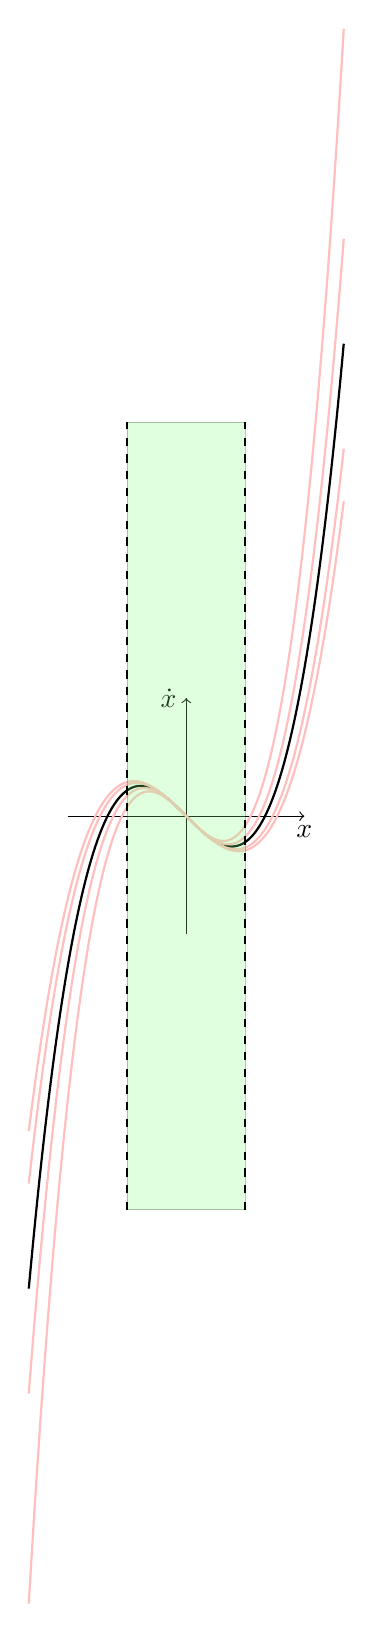
\begin{tikzpicture}[domain=-2:2,samples=400]
    \draw[->] (-1.5,0) -- (1.5,0) node[below] {$x$};
    \draw[->] (0,-1.5) -- (0,1.5) node[left] {$\dot{x}$};
    % \foreach \i in {-1,1} {
    %     \draw (\i,.1) -- (\i,-.1) node[below] {$\i$};
    % }

    % \foreach \i in {-1,1} {
    %     \draw (.1,\i) -- (-.1,\i) node[left] {$\i$};
    % }

    \draw[black, thick] plot (\x,{-\x + \x*\x*\x});

    \foreach \w in {3/4, 5/6, 7/6, 3/2} {
      \draw[pink, thick] plot(\x, {-\x + \w*\x*\x*\x});
    }

    % Fill the region of attraction
    \draw[fill=green!50, nearly transparent] (-.75,-5) -- (-.75,5) -- (.75,5) -- (.75,-5) -- cycle;

    % Draw the dashed lines around the region of attraction.
    \draw[dashed, thick, black] (-.75,-5) -- (-.75,5);
    \draw[dashed, thick, black] (.75,-5) -- (.75,5);

    % \draw[red] (-1,0) circle [radius=6pt];
    % \draw[red] (1,0) circle [radius=6pt];
    % \filldraw (0,0) circle [radius=3pt];
\end{tikzpicture}
\end{document}
  \caption{The region of attraction for the system \(\dot{x} = -x + wx^3\),
  where \(w\) is a bounded uncertainty parameter.}
\end{figure}

here the origin is still stable, but the \textit{robust region of attraction} is
smaller than it was without any uncertainty. By using the same Lyapunov
candidate as above, \(V(x) = \frac{1}{2}x^2\),
\[
  \dot{V}(x) = \frac{\partial V}{\partial x_i} f_i(x) = x(-x + wx^3) = -x^2 +
  wx^4.
\]
Which, when analyzed yields
\begin{align*}
  \dot{V}(x) &< 0 \\
  -x^2 + wx^4 &< 0 \\
  x^2 > wx^4
\end{align*}
or equivalently
\[
  \abs{x} < \frac{1}{\sqrt{w_{max}}} = \sqrt{\frac{2}{3}}.
\]
Which shows that \(\abs{x} < \sqrt{\frac{2}{3}}\) is inside the \textit{robust
  region of attraction} for the uncertain gain system.

At other times the fixed points of the uncertain system might be unknown. Still,
it is possible to employ Lyapunov functions to give guarantees about the
behaviour of the system. For this thesis this idea will be employed to stabilize
a simple vehicle model around a nominal trajectory, thus it is not so important
that the vehicle sticks exactly to the path, as long as there exists some
convergence guarantees around it.

A good example of how the fixed point is not necessary at the origin is the
\textit{Additive noise system}.

\begin{example}{Additive noise system}

  Next, consider the same system with added noise \(\dot{x} = -x + x^3 + w\),
  \(-\frac{1}{4} \leq w \leq \frac{1}{4}\). As noted previously, the fixed point
  is not at the origin for all values of \(w\), it moves depending on the value.
  However, utilizing an invariant set argument to guarantee that the the
  uncertain dynamical system will stay near the origin if it starts near the
  origin.
\end{example}


\begin{figure}
  \centering
  \documentclass[tikz,border=3mm]{standalone}
\begin{document}
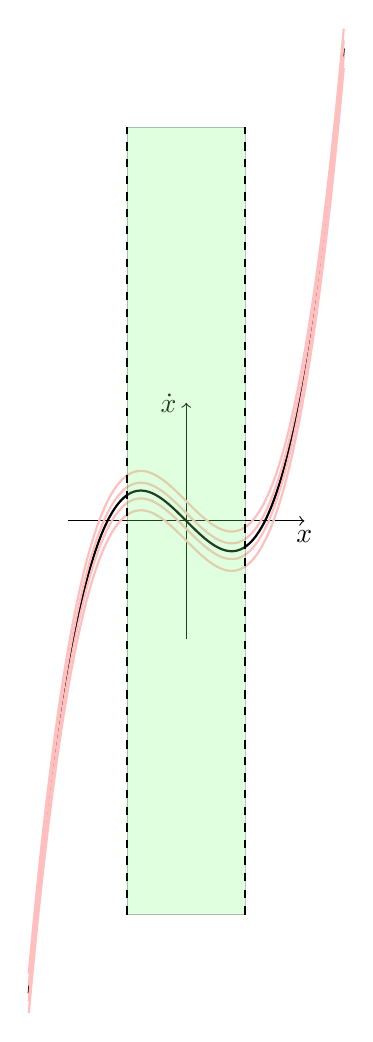
\begin{tikzpicture}[domain=-2:2,samples=400]
    \draw[->] (-1.5,0) -- (1.5,0) node[below] {$x$};
    \draw[->] (0,-1.5) -- (0,1.5) node[left] {$\dot{x}$};
    % \foreach \i in {-1,1} {
    %     \draw (\i,.1) -- (\i,-.1) node[below] {$\i$};
    % }

    % \foreach \i in {-1,1} {
    %     \draw (.1,\i) -- (-.1,\i) node[left] {$\i$};
    % }

    \draw[black, thick] plot (\x,{-\x + \x*\x*\x});

    \foreach \w in {-1/4, -1/10, 1/10, 1/4} {
      \draw[pink, thick] plot(\x, {-\x + \x*\x*\x + \w});
    }

    % Fill the region of attraction
    \draw[fill=green!50, nearly transparent] (-.75,-5) -- (-.75,5) -- (.75,5) -- (.75,-5) -- cycle;

    % Draw the dashed lines around the region of attraction.
    \draw[dashed, thick, black] (-.75,-5) -- (-.75,5);
    \draw[dashed, thick, black] (.75,-5) -- (.75,5);

    % \draw[red] (-1,0) circle [radius=6pt];
    % \draw[red] (1,0) circle [radius=6pt];
    % \filldraw (0,0) circle [radius=3pt];
\end{tikzpicture}
\end{document}
  \caption{The region of attraction for the system \(\dot{x} = -x + x^3 + w\),
    where \(w\) is a bounded uncertainty parameter.}
\end{figure}

Once again, applying the same Lyapunov function \(V(x) = \frac{1}{2}x^2\),
\[
  \dot{V}(x) = \frac{\partial V}{\partial x_i} f_i(x) = x(-x + x^3 + w) = -x^2 +
  x^3 + wx.
\]
However, the invariant set argument here is a little different, as every
sub-level set of the Lyapunov function is invariant. For instance \(V \leq
\frac{1}{3}\) is a \textit{robust invariant set}, because if \(V =
\frac{1}{3}\),
\[
  \forall w \in \left[ w_{min}, w_{max} \right], \; \dot{V}(x,w) < 0.
\]
Thus, \(V(x)\) can never start out at less than \(\frac{1}{3}\), and obtain
values greater than \(\frac{1}{3}\).
\[
  V = \frac{1}{3} \implies x = \pm \sqrt{\frac{2}{3}} \implies \dot{V} =
  -\frac{2}{9} \pm w \sqrt{\frac{2}{3}} < 0, \; \forall w \in \left[
    -\frac{1}{4}, \frac{1}{4} \right].
\]
However, note that \(V = \frac{1}{32}\) yields
\[
  V = \frac{1}{32} \implies x = \pm \frac{1}{4} \implies \dot{V} = -\frac{1}{4}
  + \frac{1}{16} \pm w\frac{1}{4}, \; \not \forall w \in \left[ -\frac{1}{4},
    \frac{1}{4} \right].
\]
Which shows that not all sub-level sets of an invariant set is invariant in the
case of additive uncertainty, so the conclusion is that it is not robustly
invariant.

Through the \ac{SOS} procedure and the Lyapunov function theory outlined, a
\ac{SOS} program for verifying the dynamical system utilized in the examples
looks like
\begin{example}{Region of attraction for the one-dimensional cubic system}
  \[
    \dot{x} = -x + x^3
  \]
  Using the Lyapunov function candidate \(V = x^2\), and the multiplier
  polynomial \(L(x) = \alpha_0 + \alpha_1x + \alpha_2x^2 + \alpha_3x^3 +
  \alpha_4x^4\), the \ac{SOS} optmization problem can be defined as

\begin{align*}
  \text{find } \alpha& \\
  \text{subject to }& -\dot{V}(x) - L(x)\left[ 1 - V(x) \right] \; &\text{is SOS} \\
                     & &L(x) \text{ is SOS}.
\end{align*}

Which written in~\cite[Yalmip]{Lofberg2004,Lofberg2009} yields

\end{example}

\begin{figure}
  \centering
  \lstinputlisting[language=matlab]{figures/preliminaries/cubicregionofattraction.m}
  \caption{TODO - fix this program.}
\end{figure}

\subsubsection{Robust set-invariance}

A sub-level set of the Lyapunov function is, in comparison with the system
without uncertainties, not guaranteed that every sub-level set of the Lyapunov
function is not necessarily invariant. (Give example.).

\subsection{Cyclic coordinates and LaGrangian dynamics}

The \funnel\'s generated in this thesis will be motion primitives for the
\rrtfunnel\ algorithm this thesis develops.


